\documentclass[11pt,a4paper]{article}
\usepackage{listings}
\usepackage{amssymb}
\usepackage{amsmath}
\usepackage[utf8]{inputenc}
\usepackage[russian]{babel}
\usepackage[margin=0.5in]{geometry}
\usepackage{graphicx}
\usepackage{listings}
\allowdisplaybreaks

\title{Лекция по АиСД №2}

\date{\today}

\author{Попов Никита}


\begin{document}
\maketitle

\section*{Двоичное дерево поиска}

Так как курс всё же называется <<Алгоритмы и \emph{структуры данных}>>, рассмотрим такую структуру данных, как \textbf{двоичное дерево поиска}.

Во-первых, это двоичное дерево --- есть узлы и связи между ними, при этом у каждого узла не более двух детей.
В вершинах дерева --- числа, при этом в левом поддереве узла все числа не больше, чем в самом узле; в правом же поддереве, наоборот, не меньше.

Введём обозначения: пусть $x$ --- некоторый узел. Тогда
\begin{itemize}
    \item $x$.key --- число в узле;
    \item $x$.left --- левый потомок;
    \item $x$.right --- правый потомок;
    \item $x$.p --- родитель.
\end{itemize}

При этом считаем, что у каждого узла есть оба наследника, но некоторые могут узлами не являться и иметь значение NULL.

Указанные выше свойства двоичного дерева поиска можно записать так:

$y\in \text{Tree($x$.left)} \implies \text{$y$.key} \leqslant \text{$x$.key}$

$y\in \text{Tree($x$.right)} \implies \text{$y$.key} \geqslant \text{$x$.key}$

\vspace{0.6cm}

Что с этим деревом можно делать? Для начала, это дерево можно обойти так, чтобы перечислить элементы в порядке возрастания:

\begin{lstlisting}
inorder_tree_walk(x)
    if x != NULL then
        inorder_tree_walk(x.left)
        output x.key
        inorder_tree_walk(x.right)
\end{lstlisting}

Сложность алгоритма --- $\Theta(n)$; каждый узел мы посещаем не более одного раза, при этом операции внутри узла занимают константное время.

Запишем алгоритм сортировки с помощью дерева:

\begin{lstlisting}
tree_sort(a)
    t := Tree()
    for x in a do
        tree_insert(x, t)
    inorder_tree_walk(t)
\end{lstlisting}

Пусть $a = [6,2,3,5,8,1]$. Тогда построение дерева может выглядеть так (может и по-другому, дерево далеко не всегда строится однозначно):

\[
\begin{array}{c|c}
    1
\includegraphics[width=8cm]{images/04_tree_1.pdf}&
    2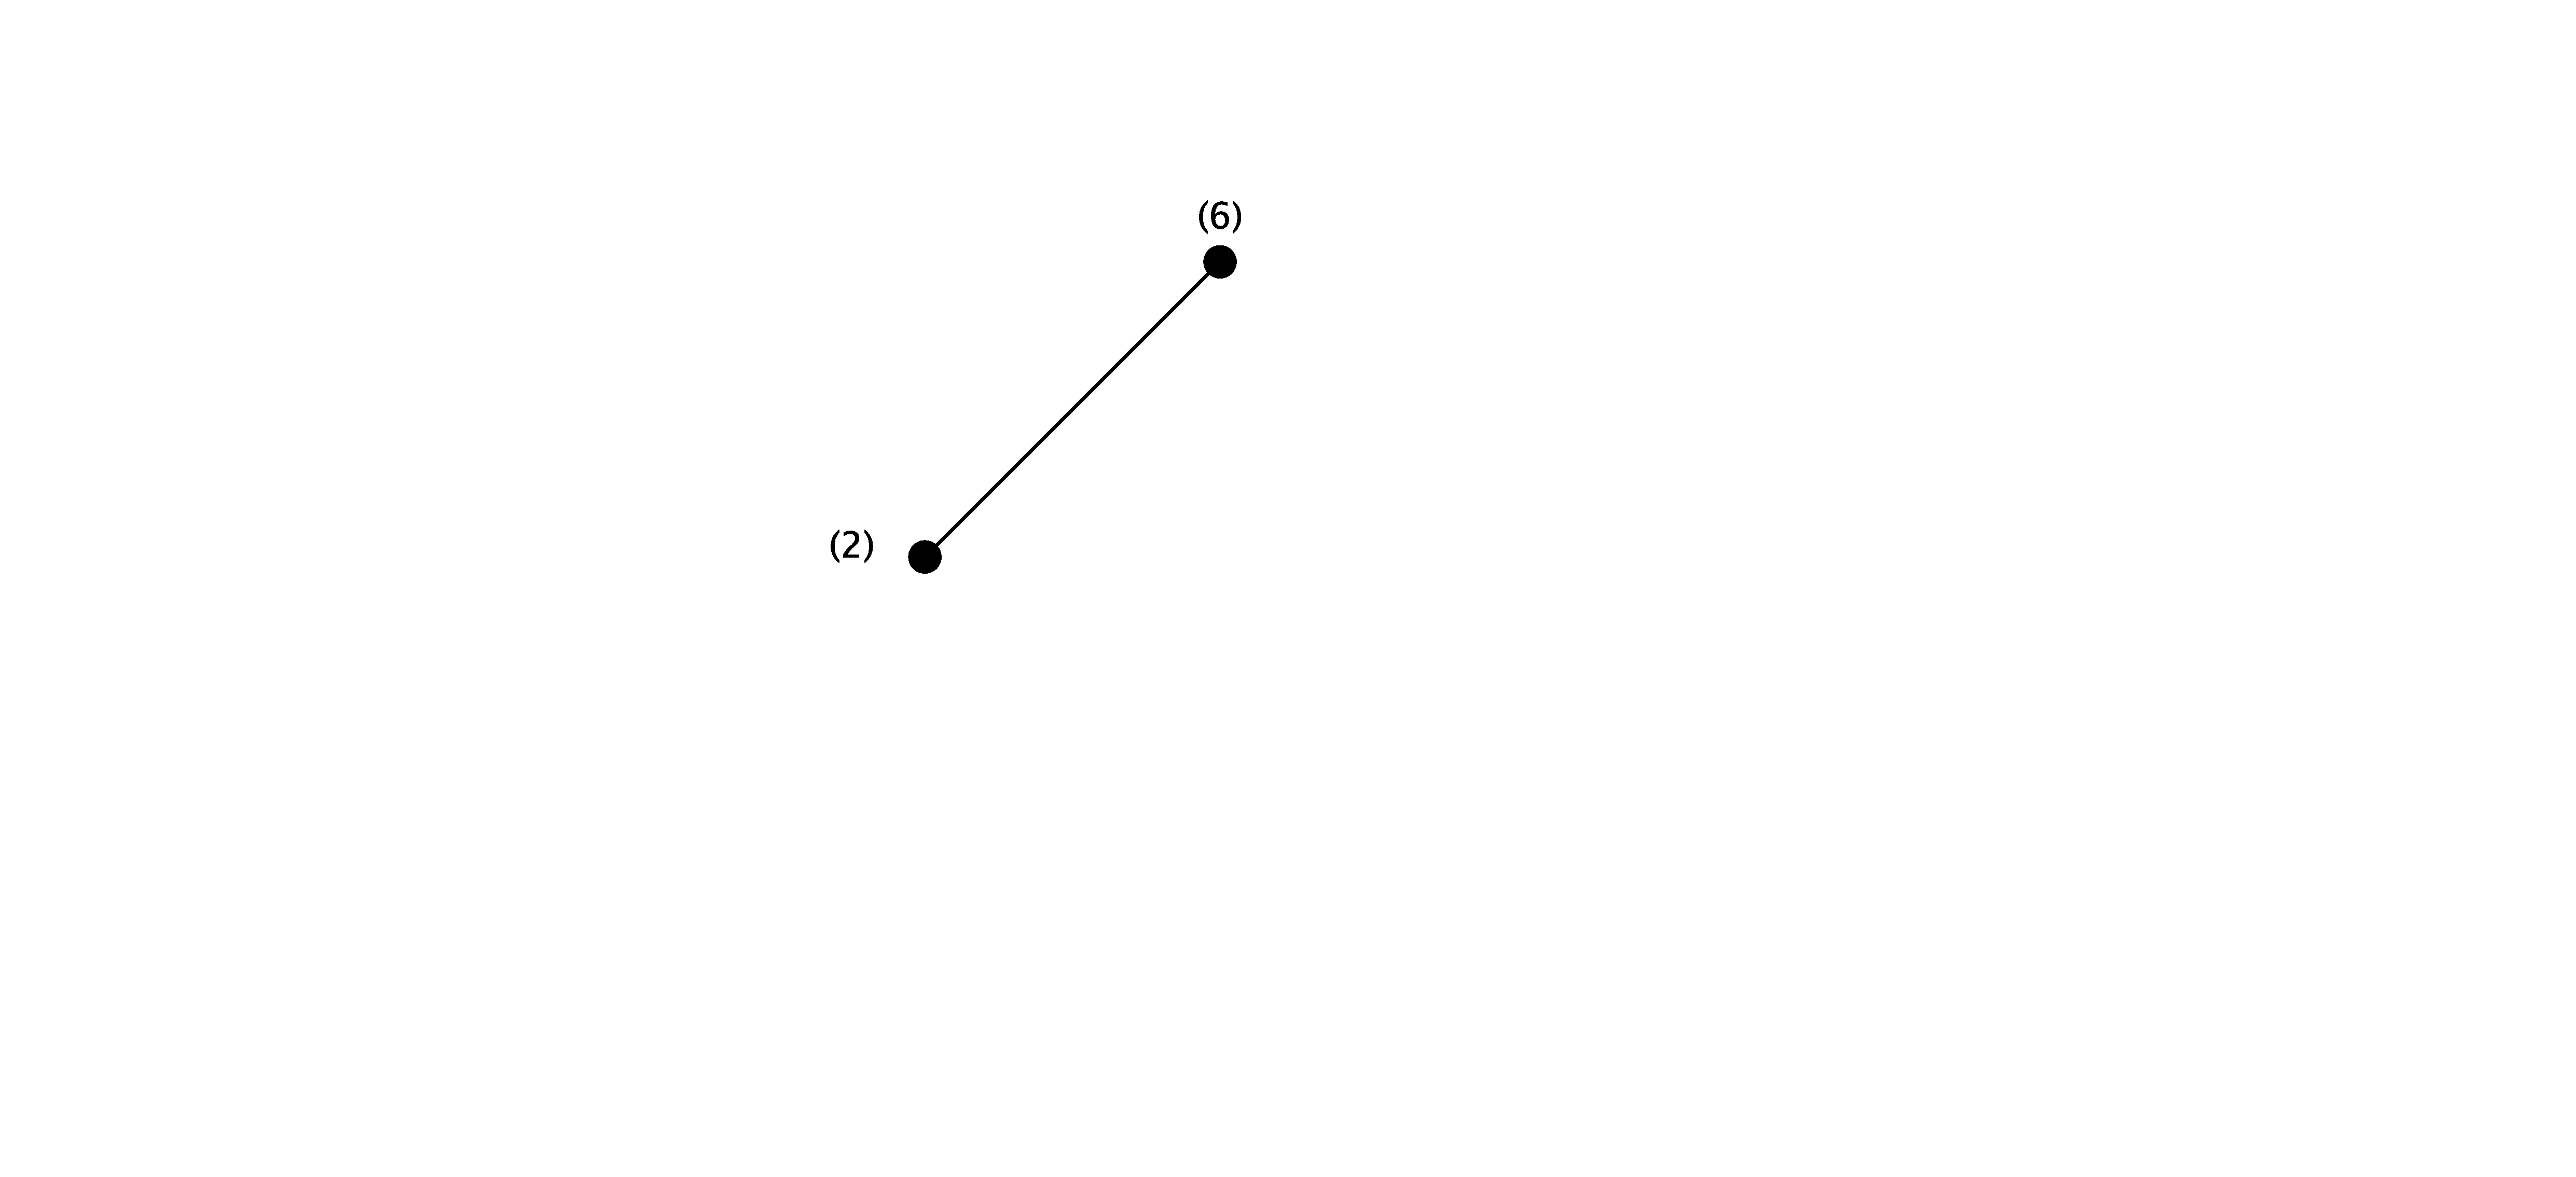
\includegraphics[width=8cm]{images/04_tree_2.pdf}\\\hline
    3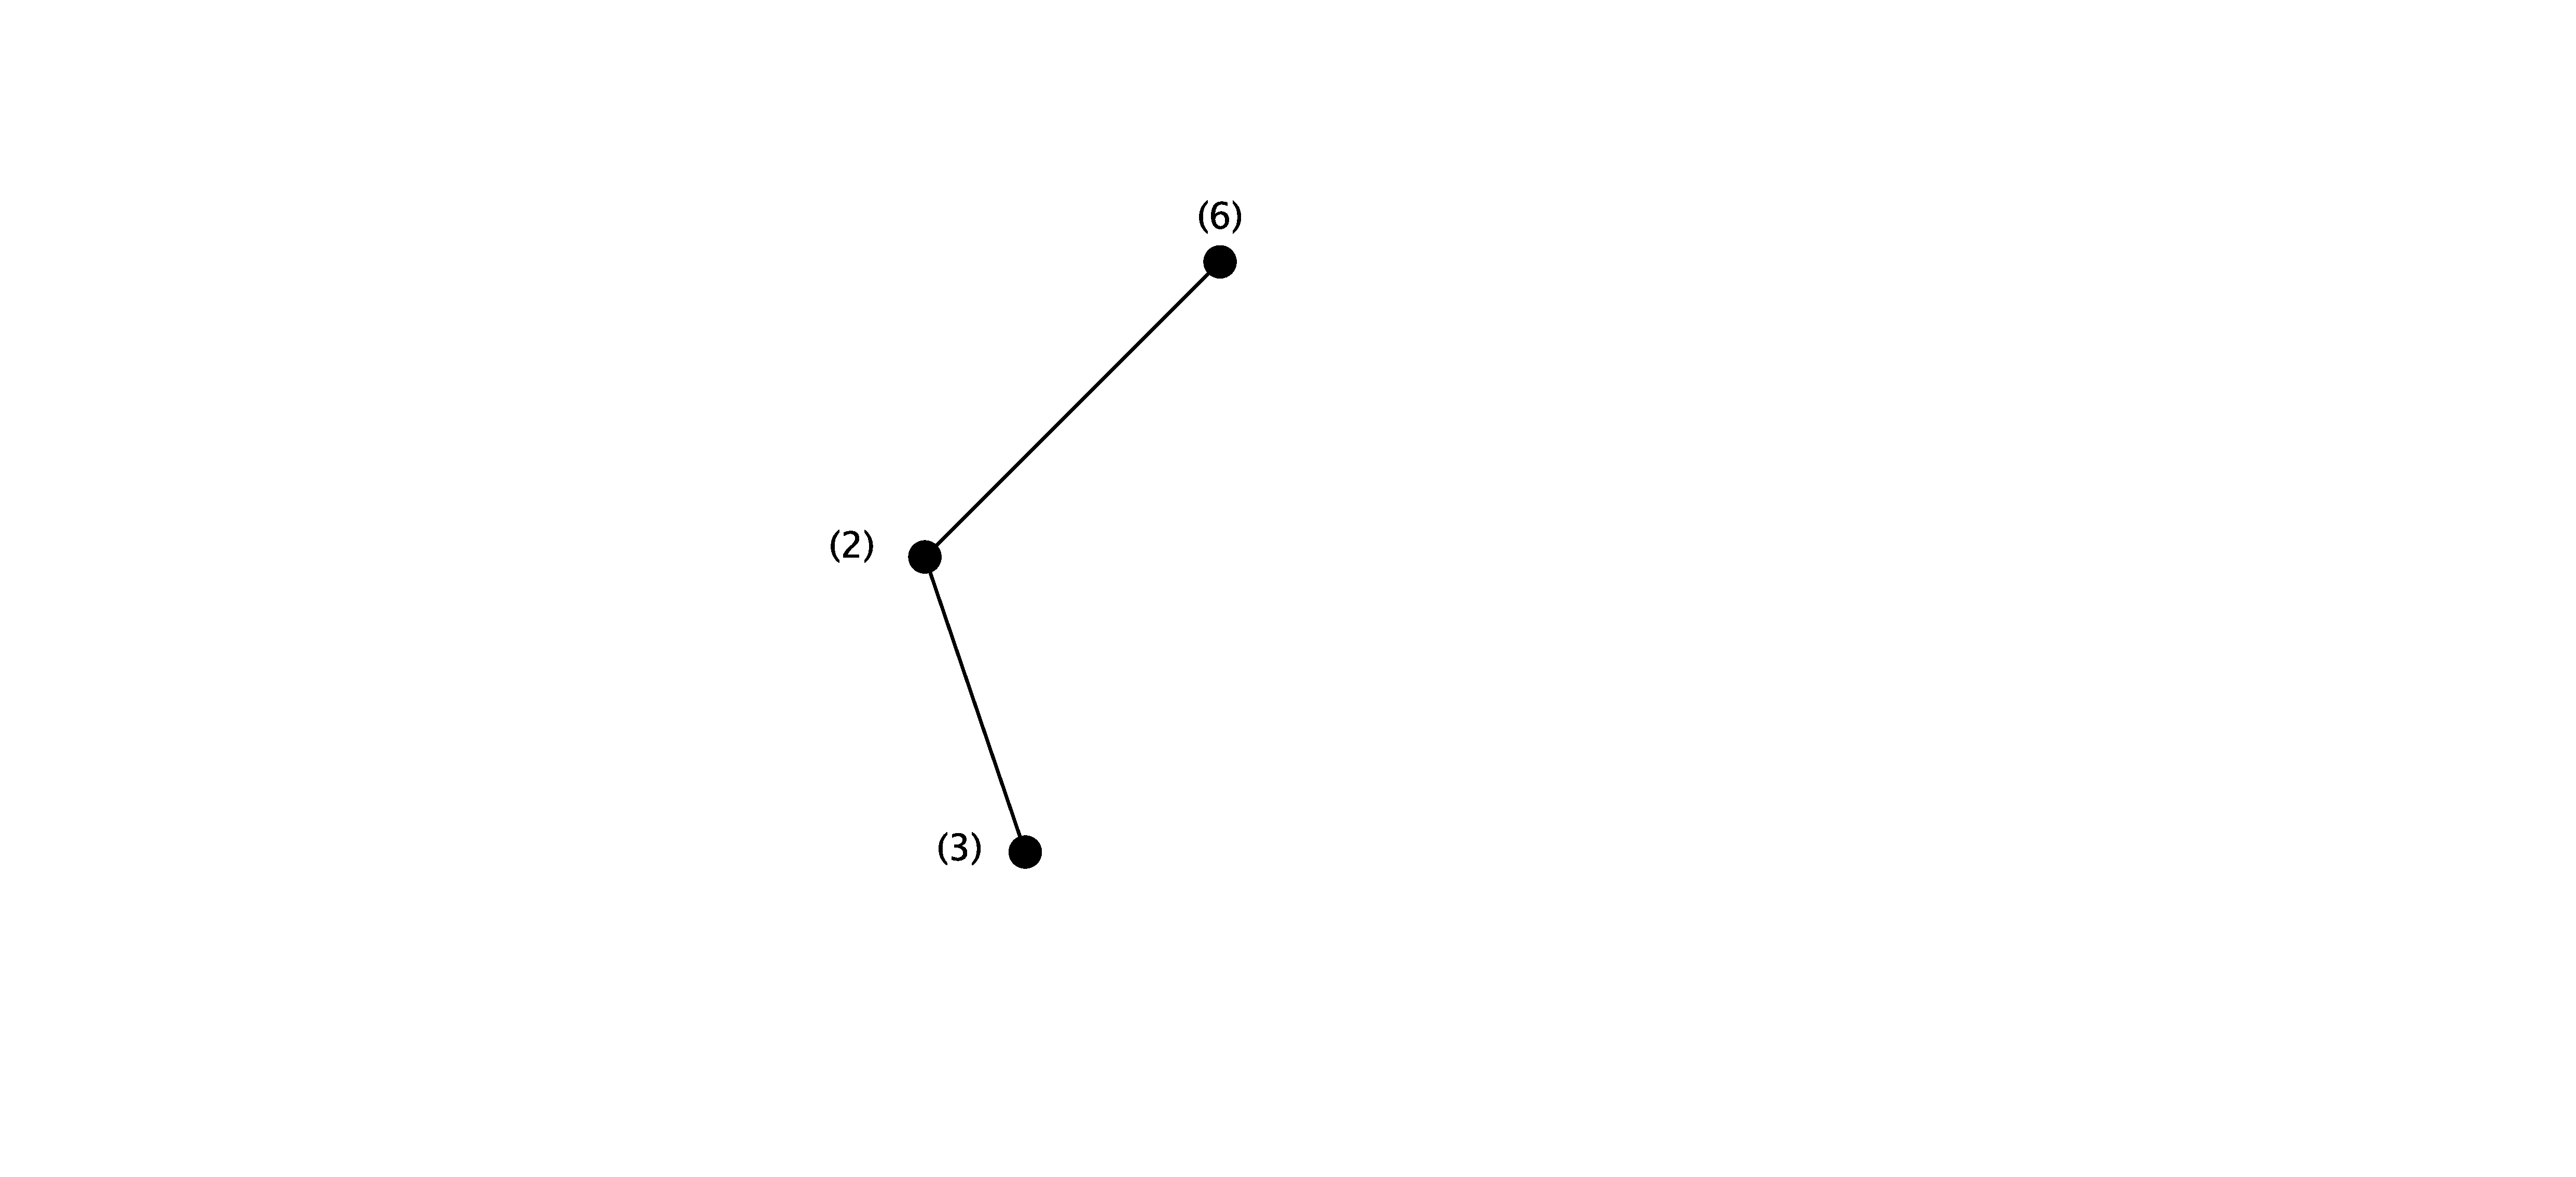
\includegraphics[width=8cm]{images/04_tree_3.pdf}&
    4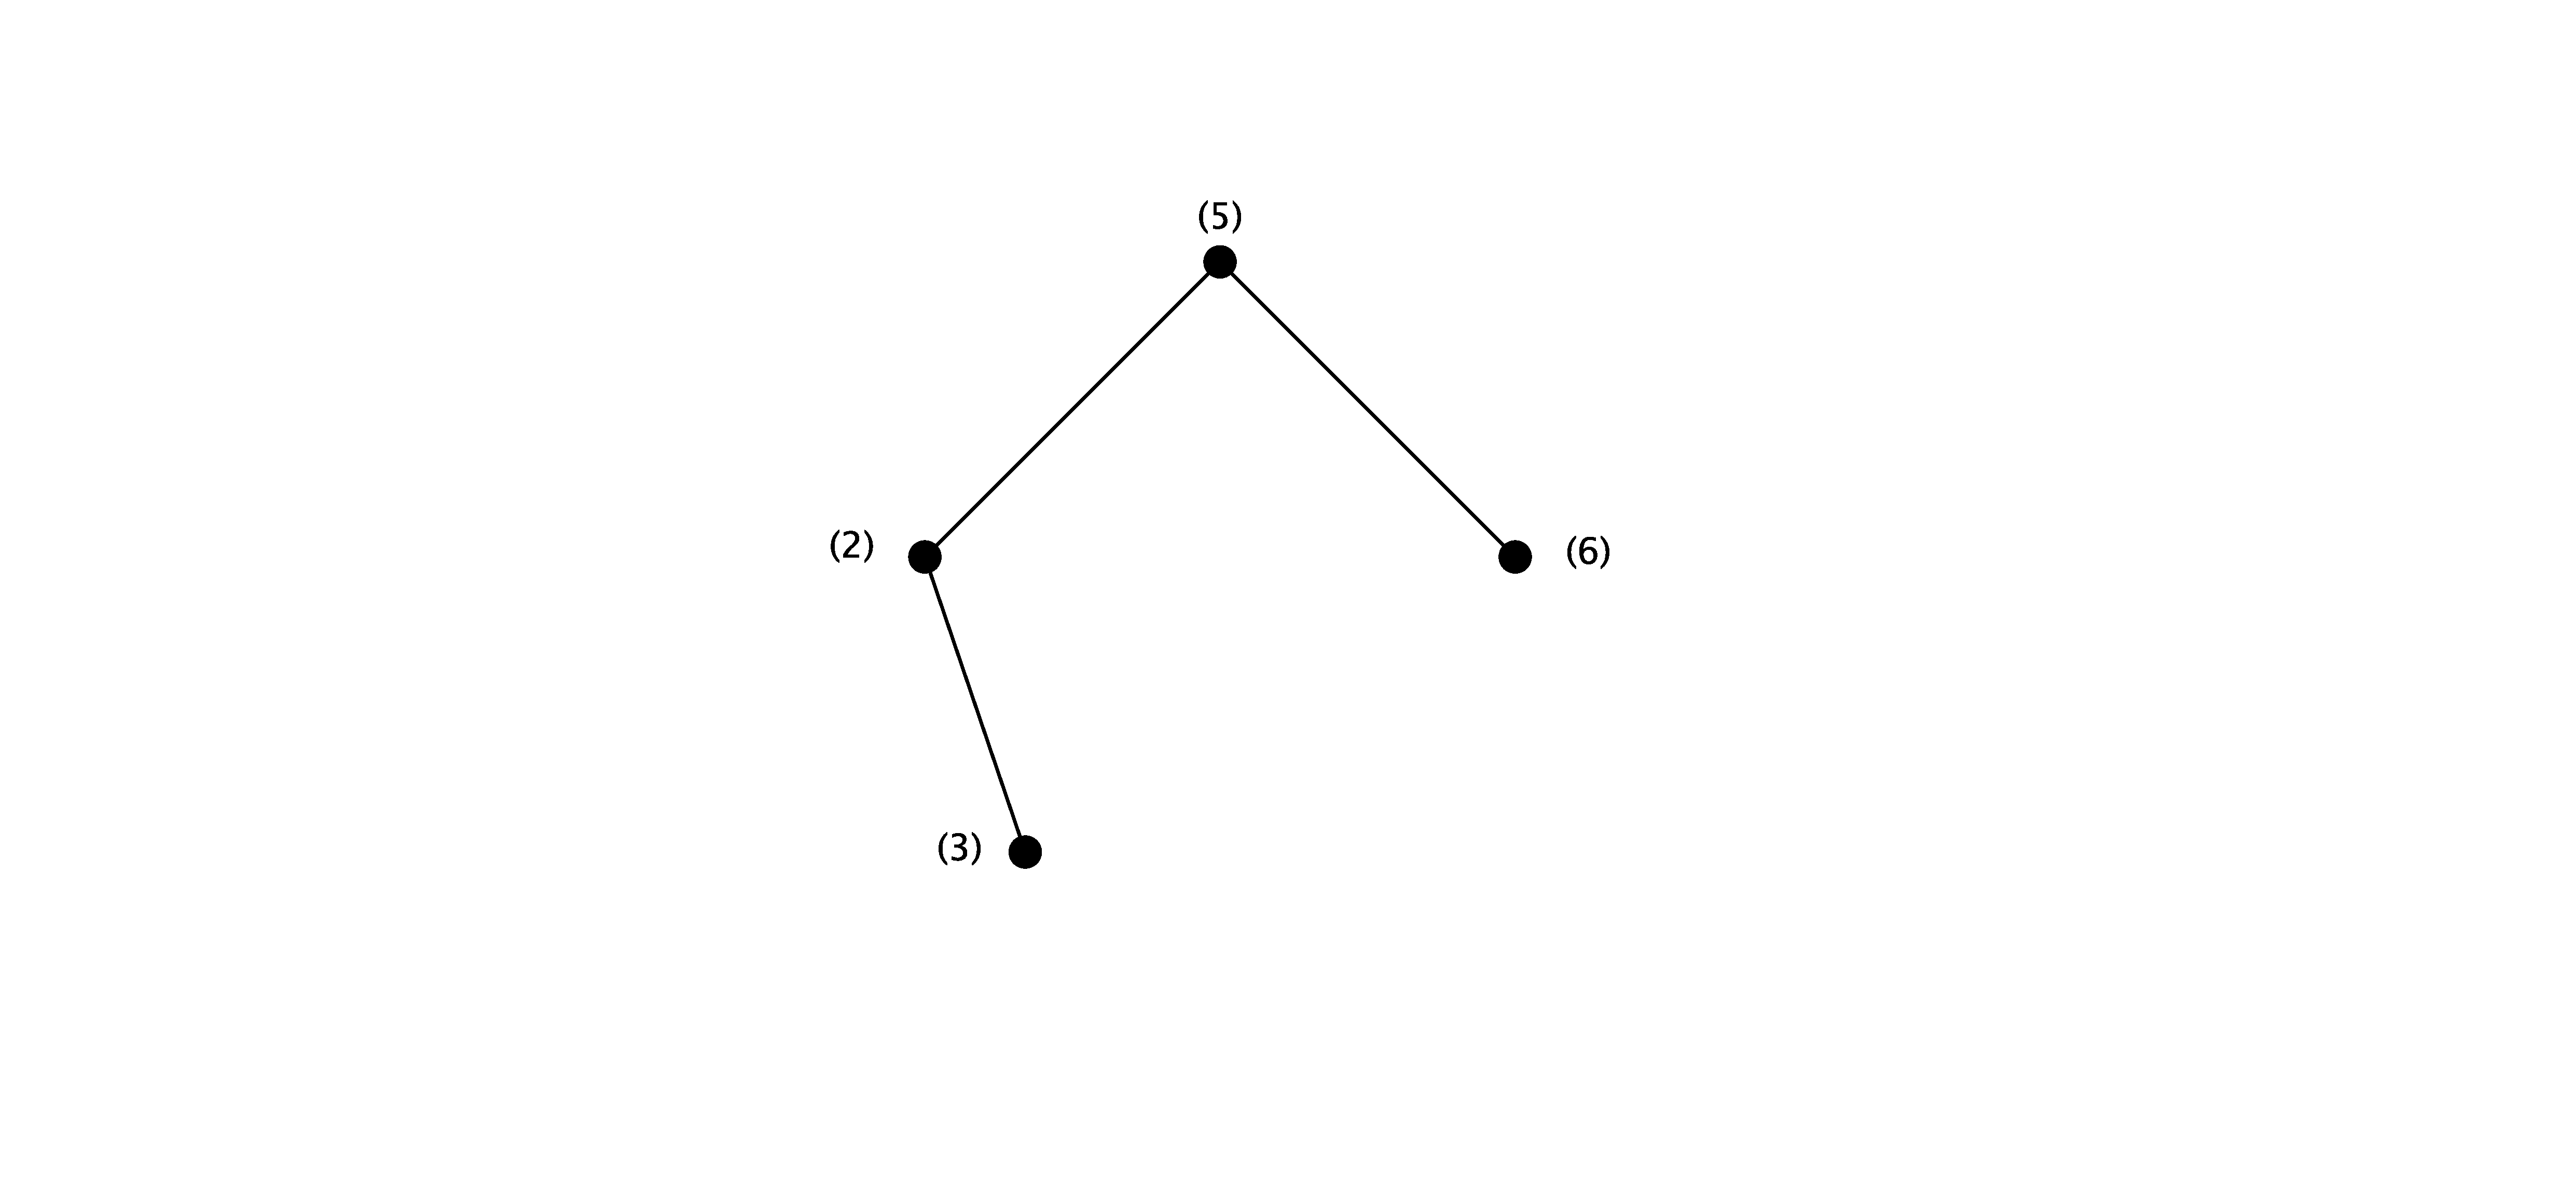
\includegraphics[width=8cm]{images/04_tree_4.pdf}\\\hline
    5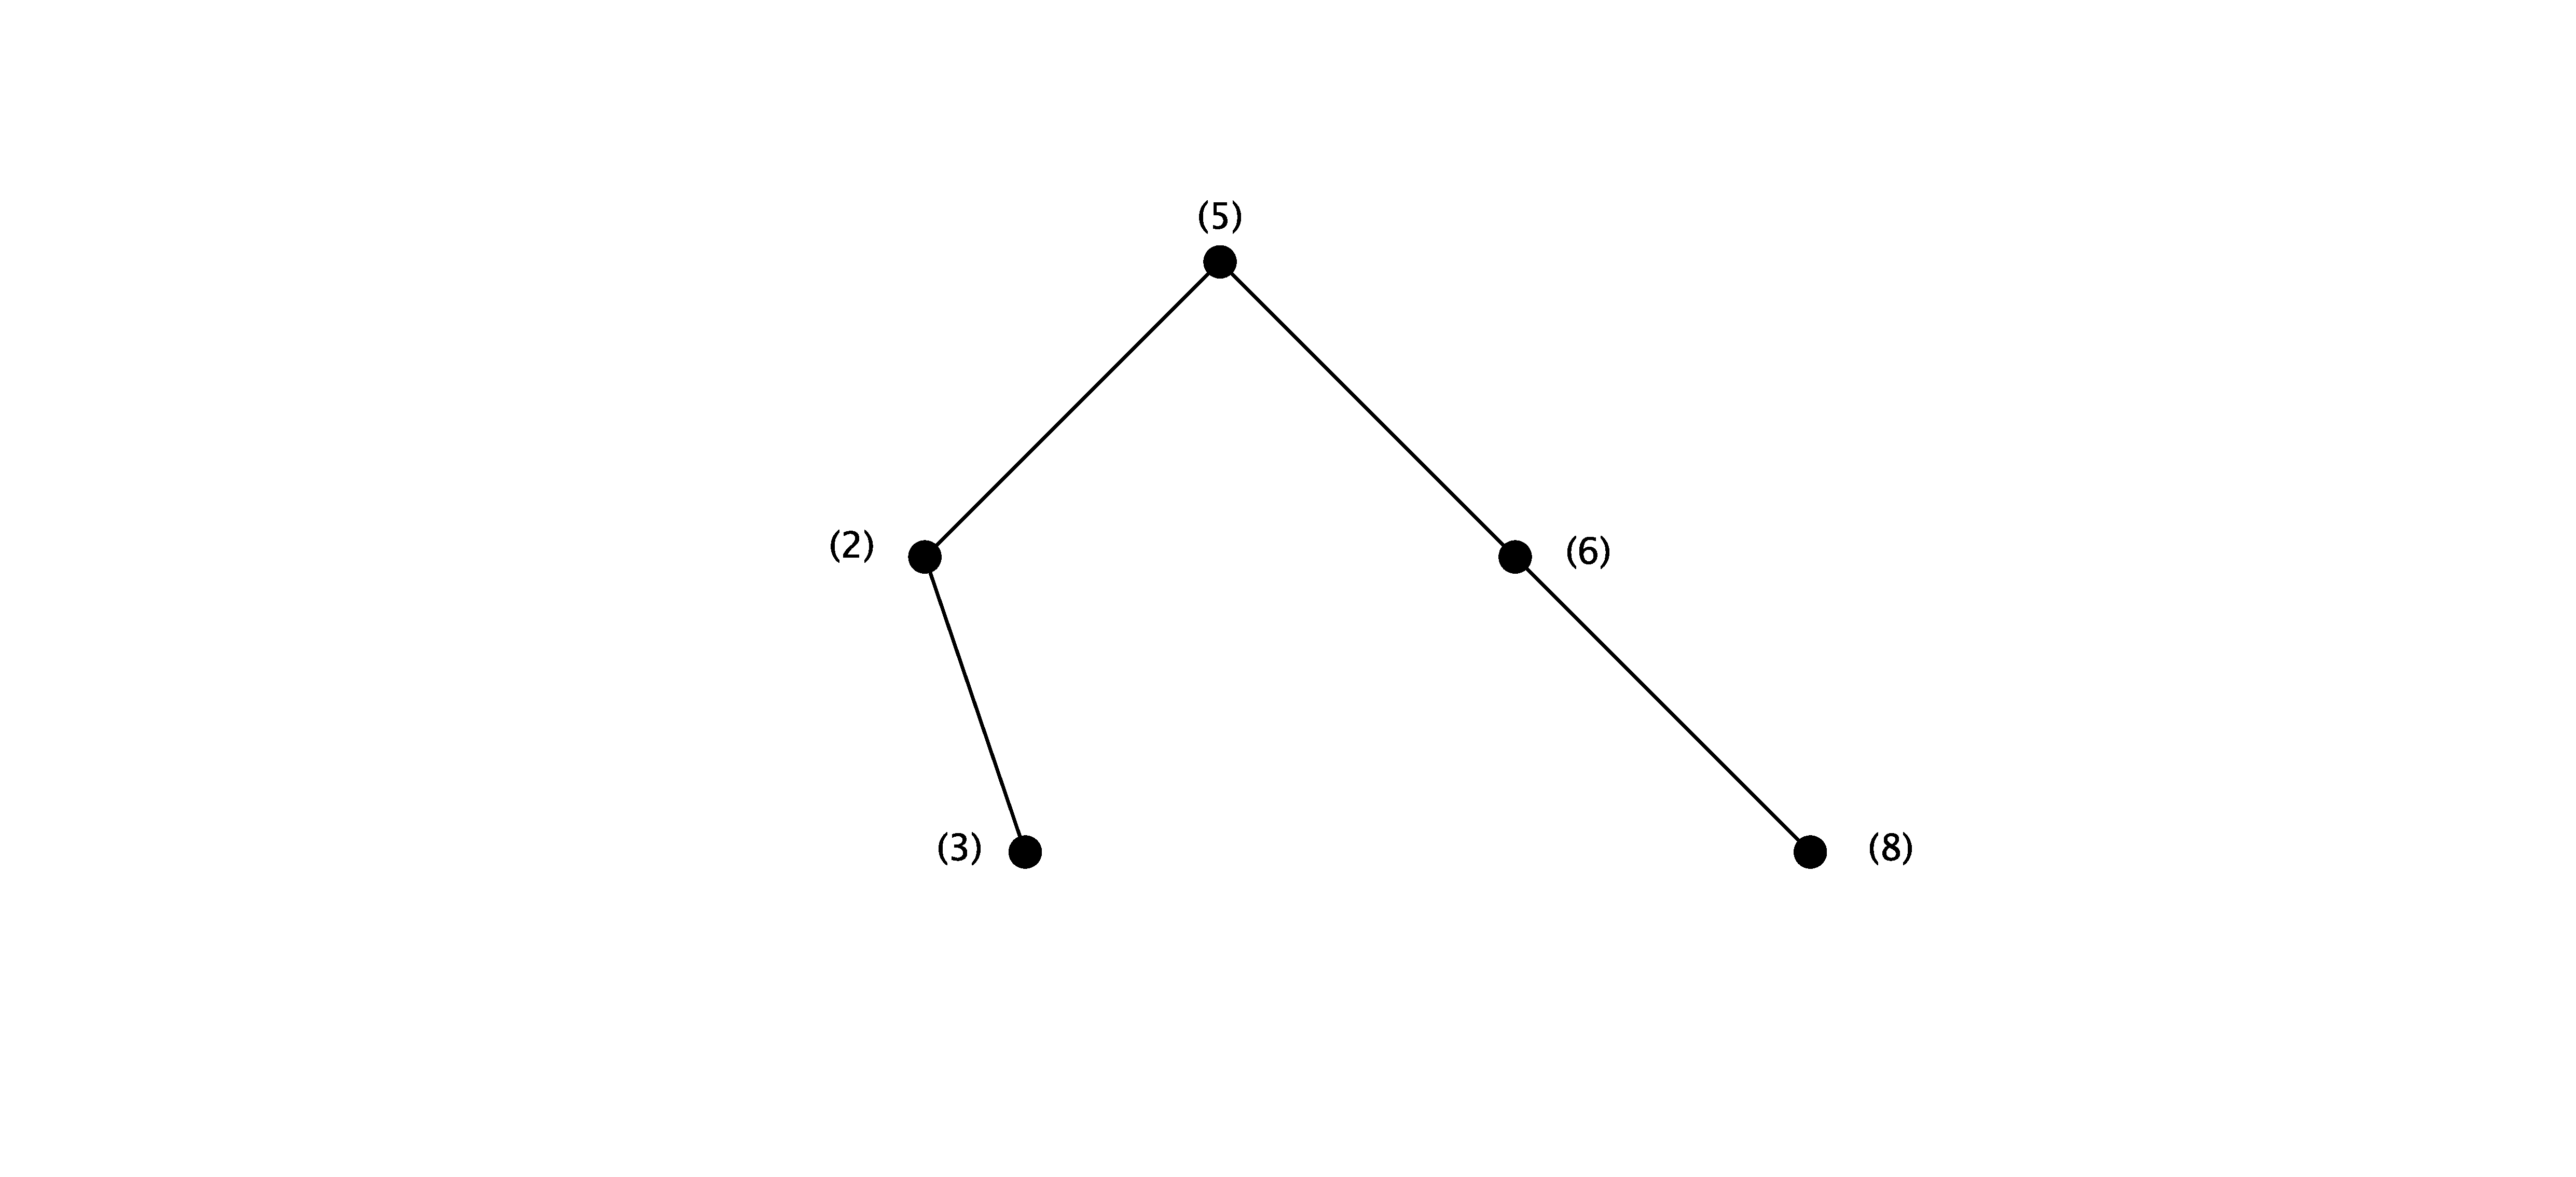
\includegraphics[width=8cm]{images/04_tree_5.pdf}&
    6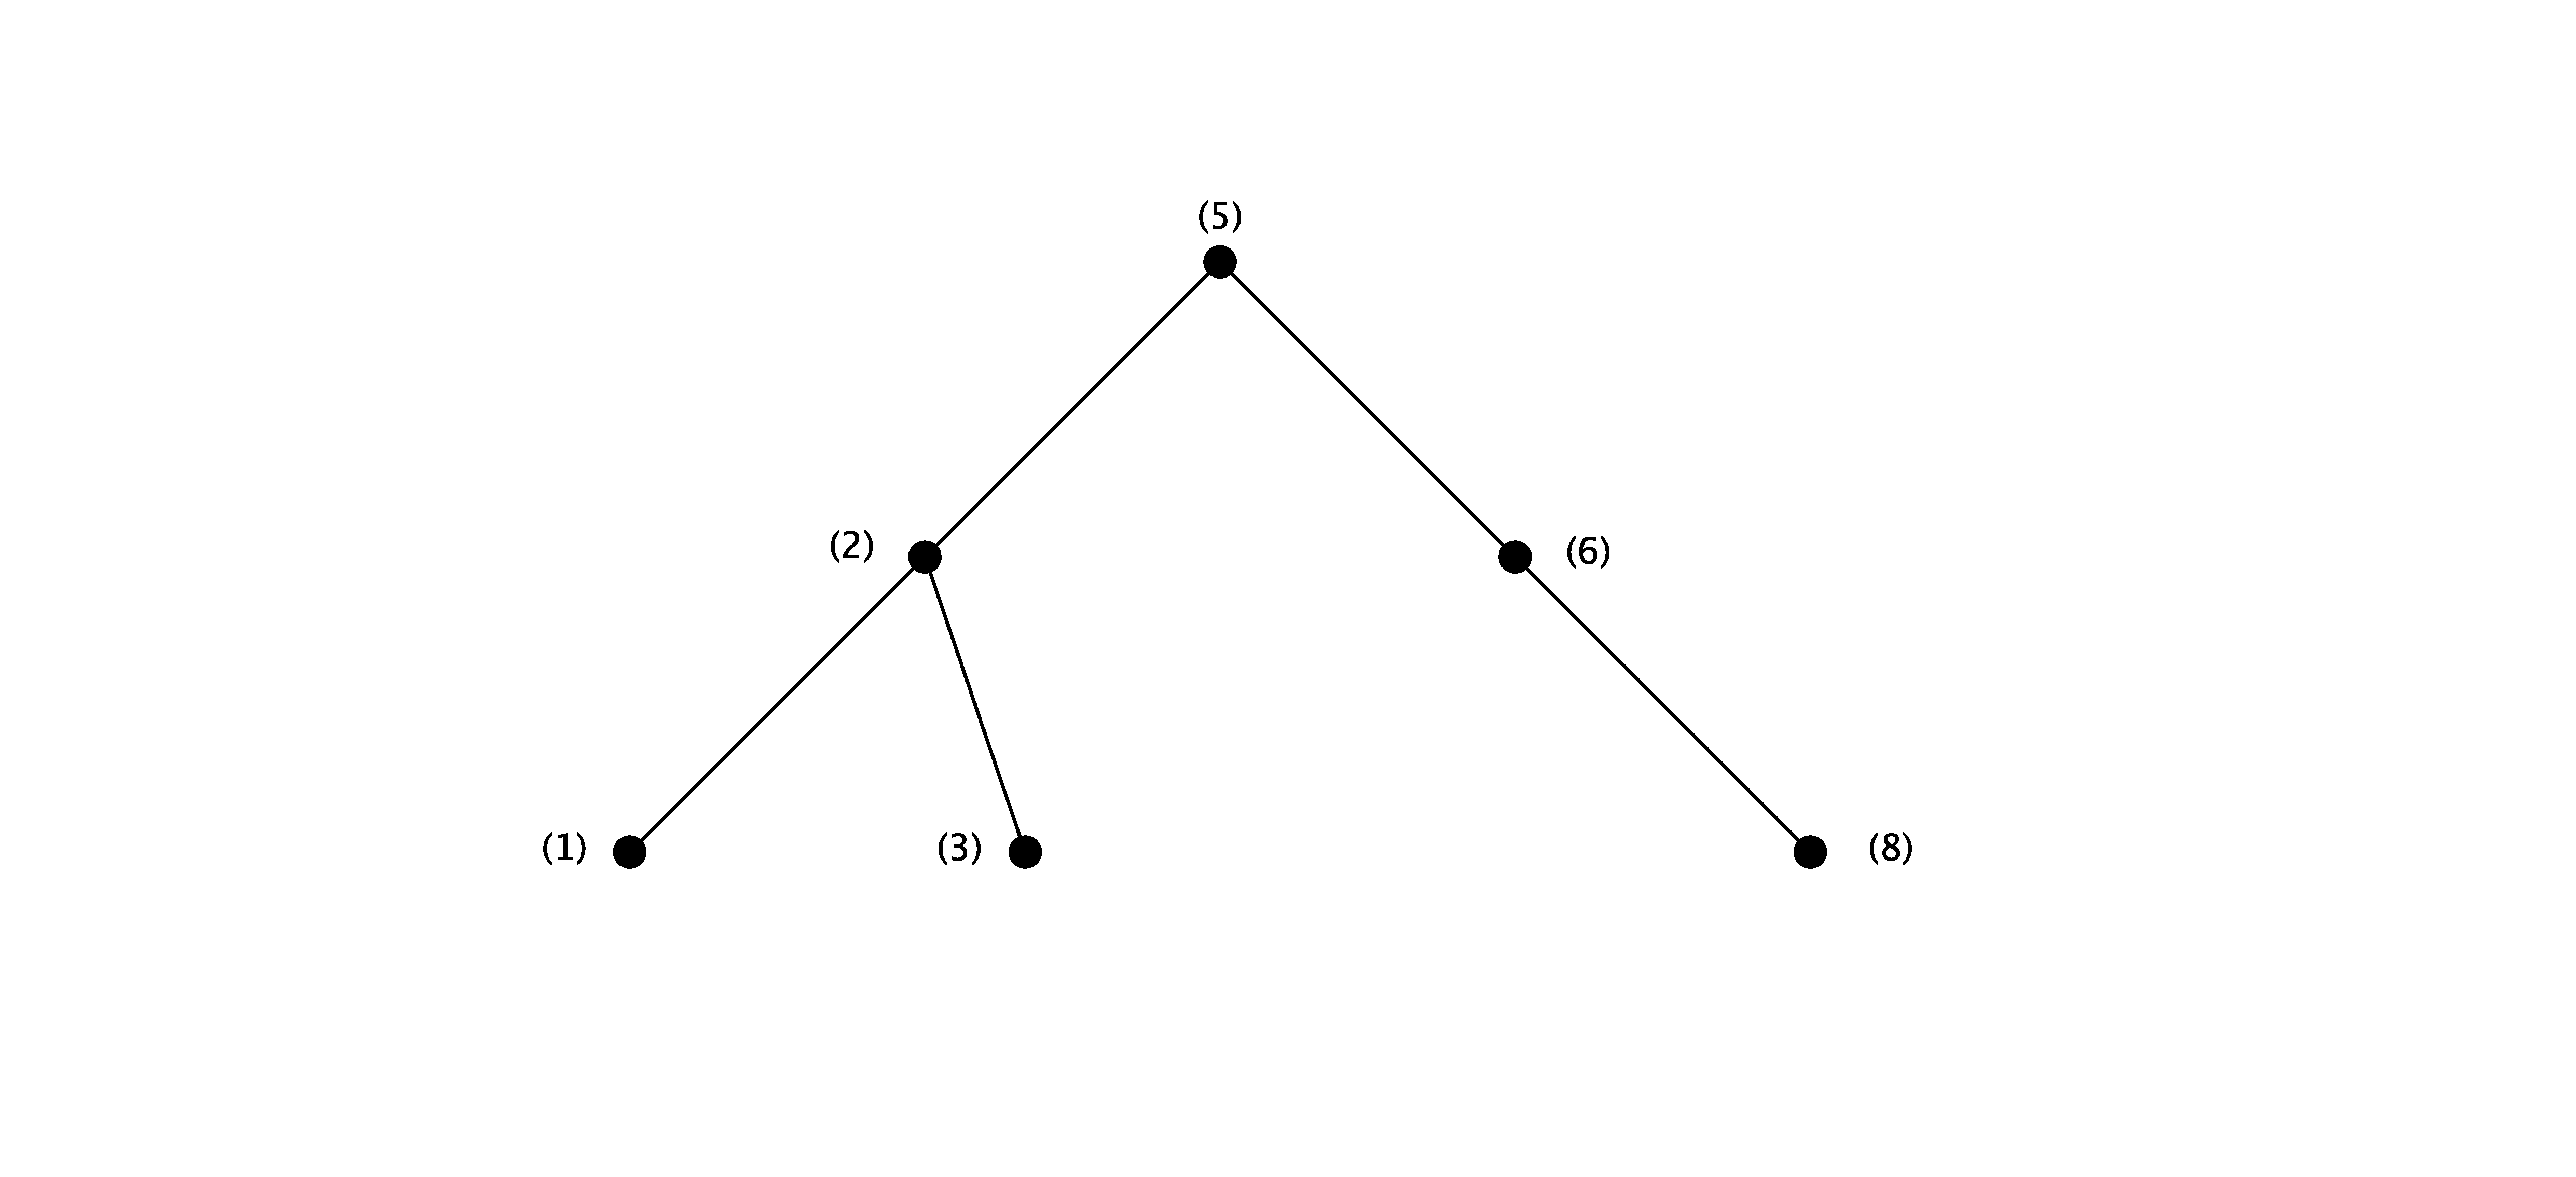
\includegraphics[width=8cm]{images/04_tree_6.pdf}
\end{array}\]

Заметим, что в общем и целом, это довольно похоже на алгоритм быстрой сортировки (особенно, если не двигать корневой элемент при вставке новых), а корень (под-)дерева --- опорный элемент.

Время работы влгоритма:
$T(n) = 2T(\frac n2) + cn \implies \Theta(n\log n)$

Предположим, что слияние дорогое:

$T(n) = 2T(\frac n2) + cn^2 \implies O(n^2 \log n)$

\vspace{1.5cm}
\textbf{HERE BE KARTINKA}
\vspace{1.5cm}

$i$-ый уровень:
\begin{itemize}
    \item Число подзадач = $2^i$
    \item Размер подзадачи = $\frac{n}{2^i}$
    \item Время на решение подзадачи = $c\left( \frac{n}{2^i} \right)^2$
    \item Всего работы = $\frac{cn^2}{2^{2i}}\cdot2^i = \frac{cn^2}{2^i}$
\end{itemize}

$T(n) \leqslant \sum\limits_{i=0}^{\log_2n-1}\frac{cn^2}{2^i} = cn^2 \sum \frac1{2^i} \leqslant2cn^2 = O(n^2)$

$T(n) = kn^d$

Удобно начинать индукцию с шага:

Пусть  $T(m)\leqslant km^d$ для $m<d$.

$T(n) \leqslant 2T(\frac n2) + cn^2 \leqslant 2k\left( \frac n2 \right)^d+cn^2 = 2k\frac{n^d}{2^d}+cn^2 = \left\{ d=2 \right\} = 2k\frac{n^2}{4} + cn^2 = \frac k2 n^2 + cn^2 = \left\{ k=2c \right\} = kn^2$

База: $T(2) \leqslant c \leqslant 2c\cdot2^2$

*я перестал понимать происходящее и переписываю формулы*

$T(n) = aT(\frac n2) + cn \implies O(n^{\log_2a})$

$T(n) \leqslant kn^d$

$T(n) = aT(\frac n2) + cn \leqslant ak \frac{n^d}{2^d}+cn = \left\{ d = \log_2a \right\} = kn^d + cn$

$T(n) \leqslant kn^d - ln$

$T(n) = aT(\frac n2) + cn \leqslant a\left(k \frac{n^d}{2^d}-l\frac n2\right)+cn = kn^d - al\frac n2 + cn = kn^d - \left( \frac{al}{2} - c \right)n = \left\{ l = \frac{al}{2} - c \right\} = kn^d - ln$

База: $T(2) \leqslant c \leqslant k\cdot 2^d - 2l$

$T(n) = T\left( \frac n2 \right) + cn$

$T(n) = \sum\limits_{i=0}^{\log_2n}c\frac{n}{2^i} = cn \sum\frac{1}{2^i} \leqslant 2cn$

Или с помощью метода частичной подстановки:

$T(n) \leqslant kn^d$

$T(n) = T\left( \frac n2 \right) + cn \leqslant \frac{kn}{2} + cn = kn^d$ аааааааааааа

\vspace{1cm}
$T(n) = aT\left( \frac nb \right) + cn^d$

\vspace{1.5cm}
\textbf{HERE BE KARTINKA}
\vspace{1.5cm}

$i$-ый уровень:
\begin{itemize}
    \item Число подзадач = $a^i$
    \item Размер подзадачи = $\frac{n}{b^i}$
    \item Время на решение подзадачи = $c\left( \frac{n}{b^i} \right)^b$
    \item Всего работы = $c\left(\frac{n}{b^i}\right)^d\cdot a^i = cn^d\left(\frac{a}{b^d}\right)^i$
\end{itemize}

Всего $\leqslant cn^d \sum\limits_{i=0}^{log_bn}\left( \frac{a}{b^d} \right)^i$
\begin{enumerate}
    \item $a = b^d$: $O(n^d\log n)$
    \item $a < b^d$: $O(n^d)$
    \item $a > b^d$: $\sum \left( \frac{a}{b^d} \right)^i = O\left( \left( \frac{a}{b^d} \right)^{log_bn} \right)$ \dots\dots\dots $O\left( n^{\log_bn} \right)$
\end{enumerate}
\end{document}
